\documentclass{beamer}

\usepackage[utf8]{inputenc}
\usepackage{color, xcolor}

% \usepackage[hidelinks]{hyperref}[citecolor=green]
% \usepackage{cite}
% \usepackage{appendix}

\usepackage{multicol}
\usepackage{fancyhdr}
\usepackage{listings}
\usepackage{graphicx, subfig}
\usepackage{float}
\usepackage{enumerate}

\usepackage{amsfonts}
\usepackage{eucal}
\usepackage{amsmath}
\usepackage{amssymb}
\usepackage{gensymb}
\usepackage{amsthm}
\usepackage{makecell}
\usepackage[ruled]{algorithm2e}
\usepackage{tikz}
\usetikzlibrary{positioning}

\usepackage[backend=bibtex,style=authoryear]{biblatex}
\bibliography{reference.bib}
\setbeamerfont{footnote}{size=\tiny}
\renewcommand{\thefootnote}{[\arabic{footnote}]}

\title{Stock Volatility Forecasting and Word Features Selection --- Based On 10-K Corpus}
\author{
  \parbox{0.3\textwidth}{
    \centering WANG Zeyu
    \vspace{.25cm}
  }
  \parbox{0.3\textwidth}{
    \centering LIU Chang
    \vspace{.25cm}
  }
  \parbox{0.3\textwidth}{
    \centering TAN Huangao
    \vspace{.25cm}
  }
  \parbox{0.3\textwidth}{
    \centering LI Borui
  }
  \parbox{0.3\textwidth}{
    \centering ZHU Xinqi
  }
  \parbox{0.3\textwidth}{
    \centering GAO Yifeng
  }
}
\date{\today}

\usetheme{Madrid}
\usecolortheme{default}
\setbeamertemplate{navigation symbols}{}

\setbeamertemplate{footline}
{
  \leavevmode%
  \hbox{%
  \begin{beamercolorbox}[wd=0.5\paperwidth,ht=2.25ex,dp=1ex,center]{author in head/foot}%
    \usebeamerfont{author in head/foot}\insertsection
  \end{beamercolorbox}%
  % \begin{beamercolorbox}[wd=.4\paperwidth,ht=2.25ex,dp=1ex,center]{title in head/foot}%
  %   \usebeamerfont{title in head/foot}\inserttitle
  % \end{beamercolorbox}%
  \begin{beamercolorbox}[wd=0.5\paperwidth,ht=2.25ex,dp=1ex,center]{date in head/foot}%
    \usebeamerfont{date in head/foot}\insertshortdate{}\hspace*{2em}
    \insertframenumber{} / \inserttotalframenumber\hspace*{2ex}
  \end{beamercolorbox}}%
  \vskip0pt%
}

\usefonttheme[onlymath]{serif}

\begin{document}

\section*{Cover}
\frame{\titlepage}

\section*{Contents}
\begin{frame}{Contents}
  \tableofcontents
\end{frame}

\section{Introduction}

\begin{frame}{Introduction - Goals}

  Our project aims to: \vspace{.25cm}
  \begin{itemize}
    \item Predict the log volatility of the following year via the MD\&A section of the Form 10-K; \vspace{.25cm}
    \item Find out the importance of each token and check whether they are similar over the years.
  \end{itemize}

\end{frame}

\begin{frame}{Introduction - Motivation}

  These two goals are meaningful because: \vspace{.25cm}

  \begin{itemize}
    \item The MD\&A section is most related to the forecasting in Form 10-K; \vspace{.25cm}
    \item A better predicting model can lead to a better portfolio; \vspace{.25cm}
    \item Such models show the market information transmission mechanisms. \vspace{.25cm}
  \end{itemize}

\end{frame}

\begin{frame}{Introduction - Dataset}

  We use a portion of the data in 10-K Corpus \footfullcite{kogan2009predicting}, including: \vspace{.25cm}

  \begin{itemize}
    \item The tokenized MD\&A sections;
          \begin{itemize}
            \item[-] (e.g. 1996.tok.tgz) \vspace{.25cm}
          \end{itemize}
    \item The log volatility in the related year.
          \begin{itemize}
            \item[-] (e.g. 1996.logvol.-12.txt, 1996.logvol.+12.txt) \vspace{.25cm}
          \end{itemize}
  \end{itemize}

\end{frame}

\section{Methods}

\begin{frame}{Methods - Lemmatization, Stemming and Stop token filter}

  We use the Natural Language Toolkit (NLTK) \footfullcite{nltk-py} as lemmatizer, stemmer and stop token filter. \vspace{.25cm}

  \begin{itemize}
    \item Some words are regarded as insignificant in text analysis;
          \begin{itemize}
            \item[-] (e.g. a, an, the, above, across) \vspace{.25cm}
          \end{itemize}
    \item Words appear in several inflected forms but with same meaning should be considered as the same;
          \begin{itemize}
            \item[-] (e.g. {achieves, achieved, achievement, achievements} $\rightarrow$ achiev) \vspace{.25cm}
          \end{itemize}
  \end{itemize}

\end{frame}

\begin{frame}{Methods - Term Frequency–Inverse Document Frequency (TF-IDF)}

  The term frequency–inverse focument frequency (TF-IDF) \footfullcite{sparck1972statistical} \footfullcite{robertson2004understanding} measures the importance of a word to a document in corpus via: \vspace{.25cm}

  $$
    \begin{aligned}
       & \text{(Term frequency)}             & \mathrm{tf}(t, d)  & = \frac{f_{t, d}}{\sum_{t^\prime \in d} f_{t^\prime, d}},                                     \\
       & \text{(Inverse document frequency)} & \mathrm{idf}(t, d) & = \log_2\left( \frac{N}{\left\vert \left\{ d: d \in D, t \in d \right\} \right\vert} \right),
    \end{aligned}
  $$ \vspace{.25cm}

  where $f_{t, d}$ is the raw count of a term $t$ in a document $d$, and $N$ is the total number of documents.

\end{frame}

\begin{frame}{Methods - Nonnegative Matrix Factorization (NMF)}

  Given a matrix $A \in \mathbb{R}^{n \times m}$, the nonnegative matrix factorization (NMF) \footfullcite{lee2000algorithms} aims to find two nonnegative matrixs $W \in \mathbb{R}^{n \times d}, H \in \mathbb{R}^{d \times m}$, where $d$ is the given number of dimension, such that \vspace{.25cm}

  $$
    A \approx W H.
  $$ \vspace{.25cm}

  The previous research \footfullcite{lee1999learning} have shown that this method is able to learn the semantic features of text.

\end{frame}

\begin{frame}{Methods - Naive Model (Baseline)}

  \begin{itemize}
    \item The naive model (or Persistence model) uses the current (or same period) value as the forecast; \vspace{.25cm}
    \item The previous research \footfullcite{beck2025mind} has shown that the naive model is better than many other complex models, especially for high-volatility time series; \vspace{.25cm}
    \item It doesn’t involve the word features or any assumptions.
  \end{itemize}

\end{frame}

\begin{frame}{Methods - Lasso/Ridge Regression \& Decision Tree}

  \begin{itemize}
    \item These models (also their extensions) are powerful in forecast and can have better performance compare with other models like heterogeneous autoregressive (HAR) models \footfullcite{liang2023forecasting} \footfullcite{li2022forecasting} \footfullcite{christensen2023machine}; \vspace{.25cm}
    \item These models are inherently interpretable, which can help us extract whether a word implies the increasing or decreasing of volatility.
  \end{itemize}

\end{frame}

\begin{frame}{Methods - Model Evaluation}

  We use mean absolute error and mean squared error to evaluate the results: \vspace{.25cm}

  $$
    \begin{aligned}
      \text{MAE}(x, \hat{x}) & = \frac{1}{N} \sum_{i=1}^N \vert x_i - \hat{x}_i \vert, \\
      \text{MSE}(x, \hat{x}) & = \frac{1}{N} \sum_{i=1}^N  (x_i - \hat{x}_i)^2.        \\
    \end{aligned}
  $$

\end{frame}

\begin{frame}{Methods - Model Evaluation}

  Given the model parameter $\beta \in \mathbb{R}^d$ and NMF components $H \in \mathbb{R}^{d \times m}$, we compute \vspace{.25cm}

  $$
    H^+ \beta = (V^T \Lambda^+ U) \beta
  $$ \vspace{.25cm}

  as the weight for each words via the pseudo inverse, where $H = U^T \Lambda V$ is the SVD and $\Lambda^+$ is the diagonal matrix consisting of the reciprocals of $H$’s singular values.

  We selected the top $1000$ words (about $1\% \sim 5\%$ of total) and check whether they are similar between different methods and years.

\end{frame}

\begin{frame}{Methods - Overview Flowchart}

  \begin{figure}
    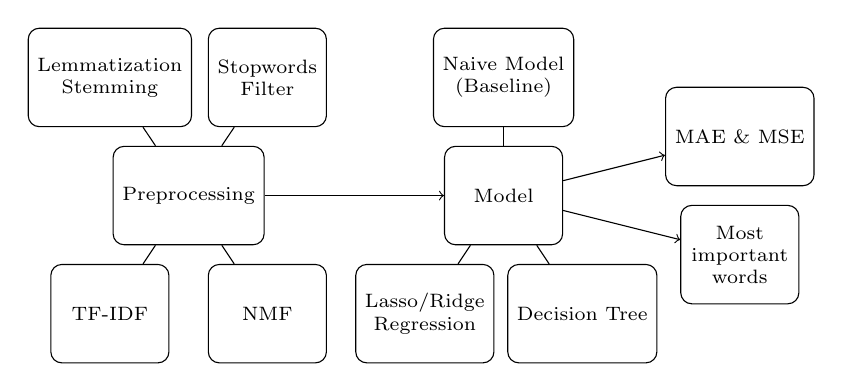
\begin{tikzpicture}[minimum width=1.5cm, minimum height=1.25cm, font=\scriptsize]
      \node[draw, align=center, rounded corners]  (P)   at ( 0,    0)    {Preprocessing};
      \node[draw, align=center, rounded corners]  (LS)  at (-1,  1.5)    {Lemmatization \\ Stemming};
      \node[draw, align=center, rounded corners]  (SF)  at ( 1,  1.5)    {Stopwords \\ Filter};
      \node[draw, align=center, rounded corners]  (T)   at (-1, -1.5)    {TF-IDF};
      \node[draw, align=center, rounded corners]  (N)   at ( 1, -1.5)    {NMF};

      \node[draw, align=center, rounded corners]  (M)   at ( 4,    0)    {Model};
      \node[draw, align=center, rounded corners]  (NM)  at ( 4,  1.5)    {Naive Model \\ (Baseline)};
      \node[draw, align=center, rounded corners]  (LR)  at ( 3, -1.5)    {Lasso/Ridge \\ Regression};
      \node[draw, align=center, rounded corners]  (D)   at ( 5, -1.5)    {Decision Tree};

      \node[draw, align=center, rounded corners]  (E)   at ( 7,  0.75)   {MAE \& MSE};
      \node[draw, align=center, rounded corners]  (W)   at ( 7, -0.75)   {Most \\ important \\ words};

      \draw[->] (P) -- (M);

      \draw[-] (P) -- (LS);
      \draw[-] (P) -- (SF);
      \draw[-] (P) -- (T);
      \draw[-] (P) -- (N);

      \draw[-] (M) -- (NM);
      \draw[-] (M) -- (LR);
      \draw[-] (M) -- (D);

      \draw[->] (M) -- (E);
      \draw[->] (M) -- (W);
    \end{tikzpicture}
  \end{figure}

  We test the model in two approaches:

  \begin{itemize}
    \item Split the data from some years into training dataset (80\%) and test dataset (20\%), and repeat the experiment to avoid flukes;
    \item Train the model via the data from some years and forecast the following year.
  \end{itemize}

\end{frame}

\section{Result}

\begin{frame}{Result - Error}

  \begin{figure}[H]
    \centering
    \includegraphics[width=0.8\textwidth]{../Result/Res-1_MAE_test.jpg} \\
    \includegraphics[width=0.8\textwidth]{../Result/Res-1_MSE_test.jpg}
    \caption{MAE and MSE for testing 1-year training set.}
  \end{figure}

\end{frame}

\begin{frame}{Result - Error}

  \begin{figure}[H]
    \centering
    \includegraphics[width=0.8\textwidth]{../Result/Res-1_MAE_pred.jpg} \\
    \includegraphics[width=0.8\textwidth]{../Result/Res-1_MSE_pred.jpg}
    \caption{MAE and MSE for predicting 1-year training set.}
  \end{figure}

\end{frame}

\begin{frame}{Result - Error}

  \begin{figure}[H]
    \centering
    \includegraphics[width=0.8\textwidth]{../Result/Res-3_MAE_test.jpg} \\
    \includegraphics[width=0.8\textwidth]{../Result/Res-3_MSE_test.jpg}
    \caption{MAE and MSE for testing 3-year training set.}
  \end{figure}

\end{frame}

\begin{frame}{Result - Error}

  \begin{figure}[H]
    \centering
    \includegraphics[width=0.8\textwidth]{../Result/Res-3_MAE_pred.jpg} \\
    \includegraphics[width=0.8\textwidth]{../Result/Res-3_MSE_pred.jpg}
    \caption{MAE and MSE for predicting 3-year training set.}
  \end{figure}

\end{frame}

\begin{frame}{Result - Word Features}

  \begin{table}[H]
    \centering
    \begin{tabular}{|c|c|c|c|}
      \hline
      Year      & Increasing Common          & Decreasing Common          & Different \\
      \hline
      1996-1997 & $53.9\%$                   & $60.6\%$                   & $1.9\%$   \\
      \hline
      1997-1998 & $35.1\%$                   & $39.2\%$                   & $6.4\%$   \\
      \hline
      1998-1999 & \textcolor{blue}{$23.6\%$} & $31.7\%$                   & $5.6\%$   \\
      \hline
      1999-2000 & \textcolor{red}{$3.8\%$}   & \textcolor{blue}{$27.8\%$} & $17.1\%$  \\
      \hline
      2000-2001 & \textcolor{red}{$5.1\%$}   & \textcolor{blue}{$24.9\%$} & $1.2\%$   \\
      \hline
      2001-2002 & $38.0\%$                   & $30.4\%$                   & $2.7\%$   \\
      \hline
      2002-2003 & $31.7\%$                   & $31.0\%$                   & $12.15\%$ \\
      \hline
      2003-2004 & \textcolor{blue}{$26.2\%$} & \textcolor{blue}{$58.3\%$} & $3.15\%$  \\
      \hline
      2004-2005 & $42.2\%$                   & $38.3\%$                   & $6.4\%$   \\
      \hline
    \end{tabular}
    \caption{Word features for lasso regression between different years.}
  \end{table}

\end{frame}

\begin{frame}{Result - Word Features}

  \begin{table}[H]
    \centering
    \begin{tabular}{|c|c|c|c|}
      \hline
      Year      & Increasing Common          & Decreasing Common          & Different \\
      \hline
      1996-1997 & $48.3\%$                   & $55.1\%$                   & $2.9\%$   \\
      \hline
      1997-1998 & $38.1\%$                   & $36.9\%$                   & $7.55\%$  \\
      \hline
      1998-1999 & \textcolor{blue}{$20.2\%$} & $32.1\%$                   & $8.35\%$  \\
      \hline
      1999-2000 & \textcolor{red}{$9.9\%$}   & $38.6\%$                   & $6.55\%$  \\
      \hline
      2000-2001 & \textcolor{red}{$13.2\%$}  & \textcolor{blue}{$18.9\%$} & $3.25\%$  \\
      \hline
      2001-2002 & $42.2\%$                   & $35.7\%$                   & $4.15\%$  \\
      \hline
      2002-2003 & $35.8\%$                   & $36.4\%$                   & $9.2\%$   \\
      \hline
      2003-2004 & \textcolor{blue}{$27.3\%$} & \textcolor{blue}{$44.6\%$} & $1.25\%$  \\
      \hline
      2004-2005 & $45.5\%$                   & $43.6\%$                   & $9.3\%$   \\
      \hline
    \end{tabular}
    \caption{Word features for ridge regression between different years.}
  \end{table}

\end{frame}

\begin{frame}{Result - Word Features}

  \begin{table}[H]
    \centering
    \begin{tabular}{|c|c|c|c|}
      \hline
      Year      & Increasing Common          & Decreasing Common        & Different \\
      \hline
      1996-1997 & $62.7\%$                   & $15.8\%$                 & $3.6\%$   \\
      \hline
      1997-1998 & $46.2\%$                   & $29.4\%$                 & $6.75\%$  \\
      \hline
      1998-1999 & $37.1\%$                   & $18.8\%$                 & $8.4\%$   \\
      \hline
      1999-2000 & $29.3\%$                   & $33.2\%$                 & $4.4\%$   \\
      \hline
      2000-2001 & $23.9\%$                   & $32.7\%$                 & $6.2\%$   \\
      \hline
      2001-2002 & $23.7\%$                   & \textcolor{red}{$3.6\%$} & $10.9\%$  \\
      \hline
      2002-2003 & $45.7\%$                   & \textcolor{red}{$5.8\%$} & $4.3\%$   \\
      \hline
      2003-2004 & \textcolor{blue}{$34.7\%$} & \textcolor{red}{$2.0\%$} & $11.85\%$ \\
      \hline
      2004-2005 & $56.7\%$                   & \textcolor{red}{$7.3\%$} & $2.1\%$   \\
      \hline
    \end{tabular}
    \caption{Word features for decision tree between different years.}
  \end{table}

\end{frame}

\begin{frame}{Result - Word Features}

  \begin{table}[H]
    \footnotesize
    \centering
    \begin{tabular}{|c|c|c|c|}
      \hline
      Year & Lasso Ridge                & Lasso DT                                     & Ridge DT                                      \\
      \hline
      1996 & $75.2\%$/$71.6\%$/$0.15\%$ & $23.2\%$/$7.7\%$/$27.0\%$                    & $36.1\%$/$25.1\%$/$17.35\%$                   \\
      \hline
      1997 & $82.0\%$/$87.2\%$/$0.15\%$ & $15.4\%$/$7.3\%$/$25.85\%$                   & $16.6\%$/$12.2\%$/$25.6\%$                    \\
      \hline
      1998 & $84.4\%$/$85.5\%$/$0.2\%$  & $14.1\%$/$15.1\%$/$15.4\%$                   & $12.2\%$/$15.6\%$/$18.6\%$                    \\
      \hline
      1999 & $67.9\%$/$83.9\%$/$0.35\%$ & $17.8\%$/$23.8\%$/$19.8\%$                   & $11.5\%$/$23.1\%$/$24.0\%$                    \\
      \hline
      2000 & $68.1\%$/$55.3\%$/$1.85\%$ & $19.0\%$/$25.1\%$/$17.6\%$                   & $24.1\%$/$9.5\%$/$26.1\%$                     \\
      \hline
      2001 & $91.7\%$/$92.9\%$/$0.1\%$  & $5.5\%$/$0.9\%$/$31.55\%$                    & $6.8\%$/$1.6\%$/$30.55\%$                     \\
      \hline
      2002 & $88.6\%$/$79.1\%$/$0.1\%$  & \textcolor{blue}{$37.7\%$/$49.8\%$/$9.75\%$} & \textcolor{blue}{$33.8\%$/$39.2\%$/$14.35\%$} \\
      \hline
      2003 & $93.6\%$/$89.5\%$/$0.15\%$ & $13.4\%$/$10.4\%$/$27.05\%$                  & $15.2\%$/$13.9\%$/$25.45\%$                   \\
      \hline
      2004 & $75.2\%$/$73.4\%$/$0.2\%$  & $23.5\%$/$24.2\%$/$21.25\%$                  & $30.4\%$/$20.4\%$/$20.85\%$                   \\
      \hline
      2005 & $95.6\%$/$90.8\%$/$0.4\%$  & $9.9\%$/$2.5\%$/$27.5\%$                     & $10.2\%$/$5.2\%$/$28.7\%$                     \\
      \hline
    \end{tabular}
    \caption{Word features between different models.}
  \end{table}

\end{frame}

\section{Conclusion}

\begin{frame}{Conclusion}

  Some conclusions are similar to the previous research \footfullcite{kogan2009predicting}:

  \begin{itemize}
    \item More training data can lead to higher accuracy and stablity; \vspace{.25cm}
    \item The Sarbanes–Oxley Act (2002) changes the information and distribution of the words; \vspace{.25cm}
    \item The Sarbanes–Oxley Act (2002) makes a higher accuracy in prediction.
  \end{itemize}

\end{frame}

\begin{frame}{Conclusion}

  For the words features: \vspace{.25cm}

  \begin{itemize}
    \item There exists the similarity between different years; \vspace{.25cm}
    \item The lasso and ridge regression always give the same features, while the decision tree chooses the different (because the decision tree is more likely to split the data based on the previous volatility); \vspace{.25cm}
    \item The abnormal during 1999 to 2001 may caused by the dot-com bubble; \vspace{.25cm}
    \item Compare with the features of increasing, the of features decreasing are more similar between years.
  \end{itemize}

\end{frame}

\section*{Reference}
\begin{frame}[allowframebreaks]{Reference}
  \printbibliography
\end{frame}

\appendix

\end{document}